% This is samplepaper.tex, a sample chapter demonstrating the
% LLNCS macro package for Springer Computer Science proceedings;
% Version 2.20 of 2017/10/04
%
\documentclass[runningheads]{llncs}
%
\usepackage{graphicx}
\usepackage{float}
\usepackage{caption}
\newcommand{\source}[1]{\caption*{Source: {#1}} }
\newcommand*{\captionsource}[2]{%
  \caption[{#1}]{%
    #1%
    \\\hspace{\linewidth}%
    \textbf{Source:} #2%
  }%
}


% Used for displaying a sample figure. If possible, figure files should
% be included in EPS format.
%
% If you use the hyperref package, please uncomment the following line
% to display URLs in blue roman font according to Springer's eBook style:
% \renewcommand\UrlFont{\color{blue}\rmfamily}

\begin{document}
%
\title{Asymmetric central pattern generator (CPG) implemented with spiking neurons in ANN (Nengo) to simulate central pattern generator (CPG) model of overground asymmetric locomotion.\thanks{Supported by Ukrainian Catholic University}}
%
%\titlerunning{Abbreviated paper title}
% If the paper title is too long for the running head, you can set
% an abbreviated paper title here
%
\author{Yuriy Pryyma\inst{1}\and
Sergiy Yakovenko\inst{2}\orcidID{0000-0002-5946-6409}}
%
% First names are abbreviated in the running head.
% If there are more than two authors, 'et al.' is used.
%
\institute{Ukrainian Catholic University
Lviv, Ukraine \and
Centers for Neuroscience, School of Medicine, West Virginia University, Morgantown, West Virginia}
%
\maketitle              % typeset the header of the contribution
%
\begin{abstract}
In this paper, we try to use a network of spiking neurons to build a Central Pattern Generator (CPG) model of a biological system. The classical approach for this problem is to build a system of ion flows inside neurons represented as several differential equations. They usually work very well but are computationally intensive. Because of this, we are limited to a shallow network of neurons and simple behavior. Spiking neural networks (SNNs) provide a more accurate version of biological neurons than Artificial neural networks(ANNs) and should be a better fit for building a model of CPGs as they are also computationally efficient.

\keywords{Asymmetric  \and CPG \and locomotion \and model \and SNN.}
\end{abstract}
%
%
%

\section{Introduction}
One of the critical properties of animals is the ability to move in a variety of environments. Locomotion as part of essential behavior shaped central neuro systems and morphologies of animals.
The central pattern generator (CPG) network is responsible for animals' rhythmic movements, and it can be formulated as a nonlinear dynamical system. The CPG model is often formulated as a differential equations system that describes ion flows inside neuron-like Hodgkin–Huxley model. Model receives low dimensional input as a command and produces a pattern of swing and stance for each of the muscles to achieve locomotion. Although biophysical models are precise, it is hard to build big networks of neurons using this approach. This work tries to validate neurobiological models of animal CPGs using spiking neural networks. They should allow abstract and more complex locomotion behavior and be of the same accuracy as biophysical models.

CPG models have a variety of applications, from limb prostheses to VR technologies. A faster and efficient limb prosthesis implemented using SNNs could work longer and improve the lives of people. 
CPGs are relatively simple parts of the brain compared to other high-level centers. Understanding of CPGs could help us better explain how our brain controls movement and be a starting point to understanding more complex behavior.


\section{Related work}
\subsection{Central pattern generator (CPG)}
Biologists often assume that vertebrate locomotion is controlled by a Central Pattern Generator (CPG) that can automatically generate complex control signals to coordinate muscles during rhythmic movements, such as walking, running, swimming, and flying. CPGs are neural networks capable of producing coordinated rhythmic activity patterns without any rhythmic inputs from sensory feedback or higher control centers. In general, locomotion organized such that CPGs are responsible for converting commands from high-level centers(the motor cortex, cerebellum) to low-level patterns of flexor and extensor movements\cite{ref1}. 

Robotics also tries to solve the problem of locomotion for robots. In the literature, there are two main approaches for the design of locomotion control systems such as kinematic and dynamic mathematical models and biologically inspired approaches\cite{ref1}. The first one tries to calculate joint speed and angel in advance, based on a mathematical model using observation for the environment and robot dynamics \cite{ref10}. The second approach tries to mimic the center of animals' locomotion and create a CPG model that will produce walking patterns. The first approach relies on a complex model and hard to adapt. Since biologists have made major advances in understanding animal locomotion, recent robotics models showed promising results with different legs configurations\cite{ref11}\cite{ref12}

There are several approaches to model CPG. The first one is detailed biophysical models. There are usually based on a system of differential equations that describe how ion pumps and ion channels influence membrane potentials and the generation of action potentials \cite{ref2} \cite{ref3} \cite{ref4}. Hodgkin–Huxley model \cite{ref1_2}(also termed H–H model) developed in the early 1950s is the most popular. However, it is very complicated and computationally expensive for computer simulations involving large populations of neurons. Because of it, most models concentrate on the detailed dynamics of small circuits. The second one uses more abstracted versions of neurons. One of the earliest models of an abstracted neuron is the integrate-and-fire model\cite{ref5}\cite{ref6}. These models focus on how a rhythmic activity is generated by network properties (e.g., half-center networks) and how different oscillatory neural circuits get synchronized via interneuron connections. The disadvantage of this model is that it implements no time-dependent memory present in natural neuron systems. Another approach is to represent CPG as a dynamical system of coupled, nonlinear oscillators. As opposite to neural oscillators, nonlinear oscillators do not have clear biological meanings. According to Junzhi Yu\cite{ref7} typical oscillator models: Matsuoka NO, Cyclic Inhibitory NO, Kuramoto Oscillator, Wilson–Cowan NO, Hopf Oscillator. \cite{ref8} \cite{ref9}



\subsection{Spiking neural networks}
The human brain has remarkable properties such as analog computation, low power consumption, fast inference, event-driven processing, online learning, and massive parallelism. SNNs model architecture tries to mimic these properties. Because spike events are sparse and have high information content, we could significantly reduce the power consumption of parts of networks that do not receive signals. \cite{ref13}  Similarly, human brains do not use all neurons simultaneously, but only regions needed for current tasks. This same advantage is maintained in hardware \cite{ref14} \cite{ref15}. Thus, it is possible to create low energy hardware based on the property that information is sparse in time and concentrated in spikes. It is one of the biggest advantages of SNNs.


Several models of spiking neurons and SNN have developed so far, e.g.: Hodgkin–Huxley’s model  \cite{ref16}; Spike Response Models\cite{ref17}\cite{ref18}; Izhikevich models \cite{ref19}. However, the vast majority of research on SNNs has been limited to very simple and shallow network architectures on relatively simple digit recognition datasets like MNIST, while only a few works report their performance on more complex standard vision datasets like CIFAR-10. The multi-layer neural architecture in the primate’s brain has inspired researchers to concentrate on the depth of ANNs instead of using shallow networks with many neurons. Theoretical and experimental results show better performance of deep rather than wide structures. This inspired research of deep SNNs. Despite their recent success in image processing tasks using similar CNN architecture, they still cannot beat the corresponding SOTA results of DNN models. One could argue that datasets used for evaluation are more suitable for the DNNs model as they work on frame-level, unlike the SNNs model that require preprocessing frames to spikes data.

Nevertheless, the biggest problem for deep SNNs is the training process. Because spikes signals are sparse and not differentiable, we can not apply backpropagation to train a model. There exist three ways for SNN learning: 1) unsupervised learning such as spike timing-dependent plasticity (STDP); 2) indirect supervised learning such as ANNs-to-SNNs conversion; 3) direct supervised learning such as gradient descent-based backpropagation. However, by far, most of them limited to very shallow structures (network layer less than 4) or toy small datasets (e.g., MNIST, Iris), and little work points to direct training deep SNNs due to their challenges. There is work in progress to develop practical learning algorithms and efficient programming frameworks.\cite{ref20}

Research of CPG models using spiking neural networks(SNNs) mostly focused on the robotics domain to create a locomotion model for different robots. The primary motivation for using SNNs is to reduce the power consumption of embedded devices used to run the robot. Some approaches use Christiansen Grammar Evolution to estimate the spiking neural network's weights and synaptic connections and deploy the FPGA model (Field Programmable Gate Array), which shows excellent performance gains.\cite{ref21} Reinforcement based stochastic weight update could also be used to train on SNNs that runs on a lightweight raspberry pi(\cite{ref22}. The authors' model converges to the desired bio-observed tripod in 70\% of the cases, while in other cases, it converges to suboptimal gaits that can still enable the locomotion. Some of the research focus more on engendering and deployment of SNNs on specific hardware as SpiNNaker boards and do not describe the model learning process \cite{ref23} \cite{ref24}.

\subsection{Research focus}
Most of the work related to SNNs and CPG are related to robotics and hardware implementation. We are solving the problem of effective locomotion. The motivation of the work is to build neurobiological models of animal CPGs using spiking neural networks. Instead of learning parameters using evolution strategies or reinforcement learning to build an efficient robot, this is a supervised learning task to build close to a biological system. The resulting model should be comparable with real biological CPGs and other low-level models like H-H or integrate-and-fire models. 

\section{Problem Setting and Approach to Solution}
CPGs are self-sufficient networks that could produce output without any sensory input signal. They receive orders from the higher-order system(Corebal cortex, Basal ganglia). The expected speed of locomotion or types of gaits passed to CPG that converts it to produce a muscle phase pattern that achieves the required motion without the supervision of conciseness as shown in Fig.~\ref{fig2}. These patterns are then stable in time till later commands are received. Signals from environmental sensors could alter flexor and extensor phase patterns without intervention from higher-order systems. For example, we could walk without thinking about moving each muscle and avoid minor obstacles reflexively.

\begin{figure}
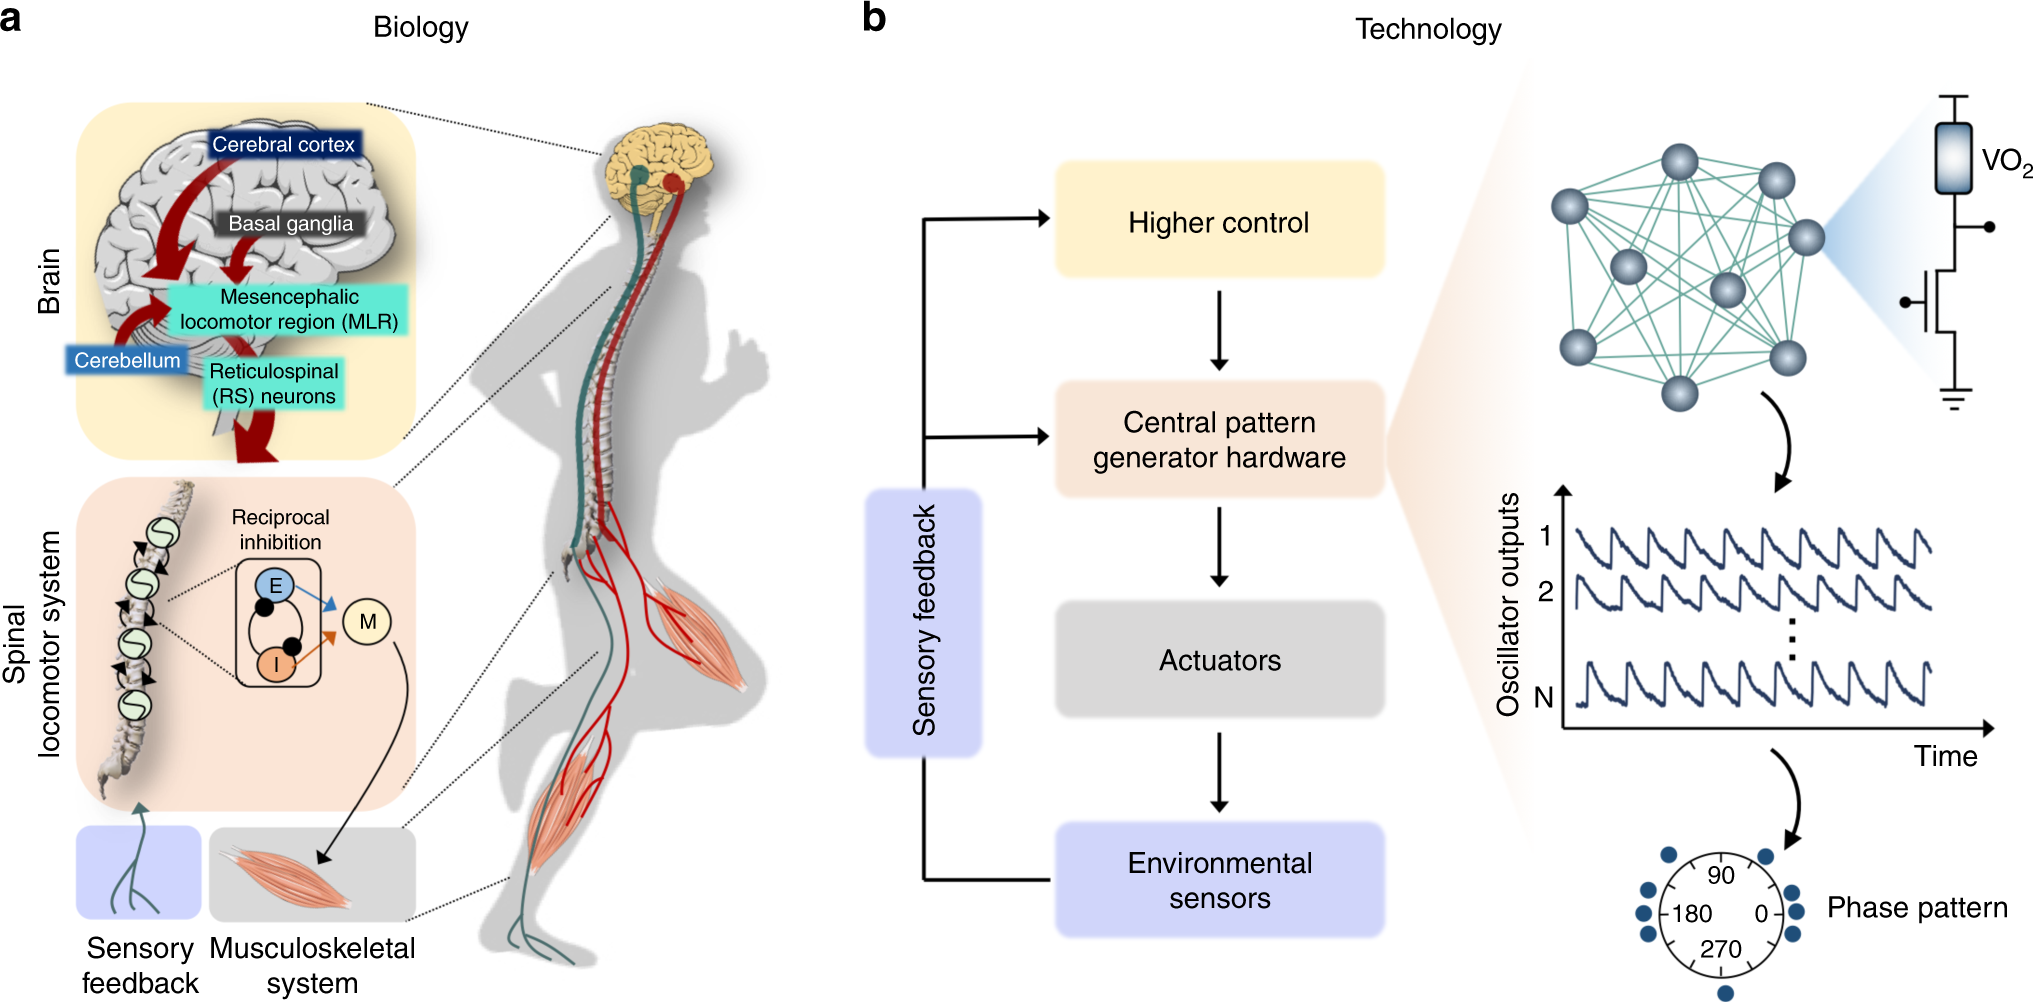
\includegraphics[width=\textwidth]{images/cpg_img.png}

\captionsource{Human locomotion system}{ https://www.nature.com/articles/s41467-019-11198-6/figures/1} \label{fig2}

\end{figure}

The movement of the animal, for example, cat, can be described as a sequence of phases stance and swing for limbs, where the stance is the duration of contact with the surface, and swing is the time in the air. As an animal moves faster, this cycle of phases shortens. Research by Halbertsma \cite{ref24_1} showed that it was mainly achieved by a decrease in stance duration while swing duration stayed mostly unchanged(example Fig.~\ref{fig3} ). Because phase-duration characteristics are integral property of motion initial test for synthetic CPG is to meet the same properties.

\begin{figure}
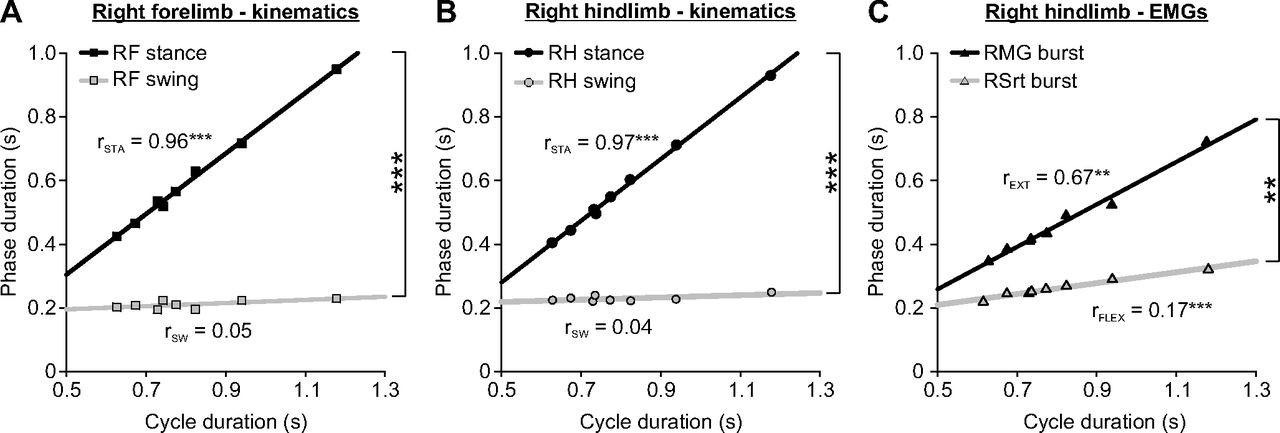
\includegraphics[width=\textwidth]{images/images_large_z9k0091424000003.jpeg}

\captionsource{Phase-duration characteristic}{ https://journals.physiology.org/cms/10.1152/jn.00524.2013/asset/images/large/z9k0091424000003.jpeg} \label{fig3}

\end{figure}


The task is to create a model that receives low dimensional input like the desired speed of an animal and produces a never-ending pattern in the same way that biological CPG does. We will use an average of 1000 steps from 9 different rats for the training and validation, which take up to 100 Gb of memory. The optimization task is to minimize the difference between real rat muscle neuron activation and generated one. Nengo framework will be used to build the CPGs model using SNNs. Spiking models are asynchronous, so input data has a time dimension. There are two ways data could be represented. In the first one, some random synchronized patterns with encoded speed will always feed to the network. Another approach would only give speed change signals once needed and empty signal any other time. There are also different approaches to train SNNs network. The research hypotheses is that SNNs could generalize well to biological CPGs.

Plan for this project:

\begin{itemize}
	\item Build an image classifier using the SNNs model to validate correctness of the Nengo framework.
	\item Build a small 4 neuron CPG base model using differential equations that optimizes phase-duration characteristics
	\item Create a SNNs networks that produces 4 signals output similar to baseline model
	\item Optimize SNNs for phase-duration characteristics and compere the results
	\item Optimize SNNs to match output data from rats dataset given different input speeds.   
	\item Expand the model input parameter to different gaits types 
	\item Measure model performance
	\item Research similarities between neurons activation of baseline model and SNNs 
\end{itemize}

\section{Early Results and Discussion}
\subsection{SNNs mnist classification using Nengo}
 Neural Engineering Object (Nengo) is a graphical and scripting software for simulating large-scale neural systems. As Neural network software, Nengo is a tool for modeling neural networks with cognitive science, psychology, Artificial Intelligence, and neuroscience applications. The first step in research would be to get familiar with the Nengo framework and do MNIST image classification using SNNs. Official tutorials could be used \cite{ref25}. SNN network, similarly to Keras functional API, could be constructed using spiking neuron network layers from Nengo. One of the be biggest concerns is how to encode two-dimensional MNIST images in time. Most often, one could copy the input signal through time simulation. Because SNNs can not be directly trained using backpropagation, Nengo automatically creates a differentiated proxy function that represents spiking neurons as done in this paper\cite{ref26}.
The final model achieves 98\% accuracy on the MNIST test dataset, on the Fig.~\ref{fig4} you could see inference example.

\begin{figure}
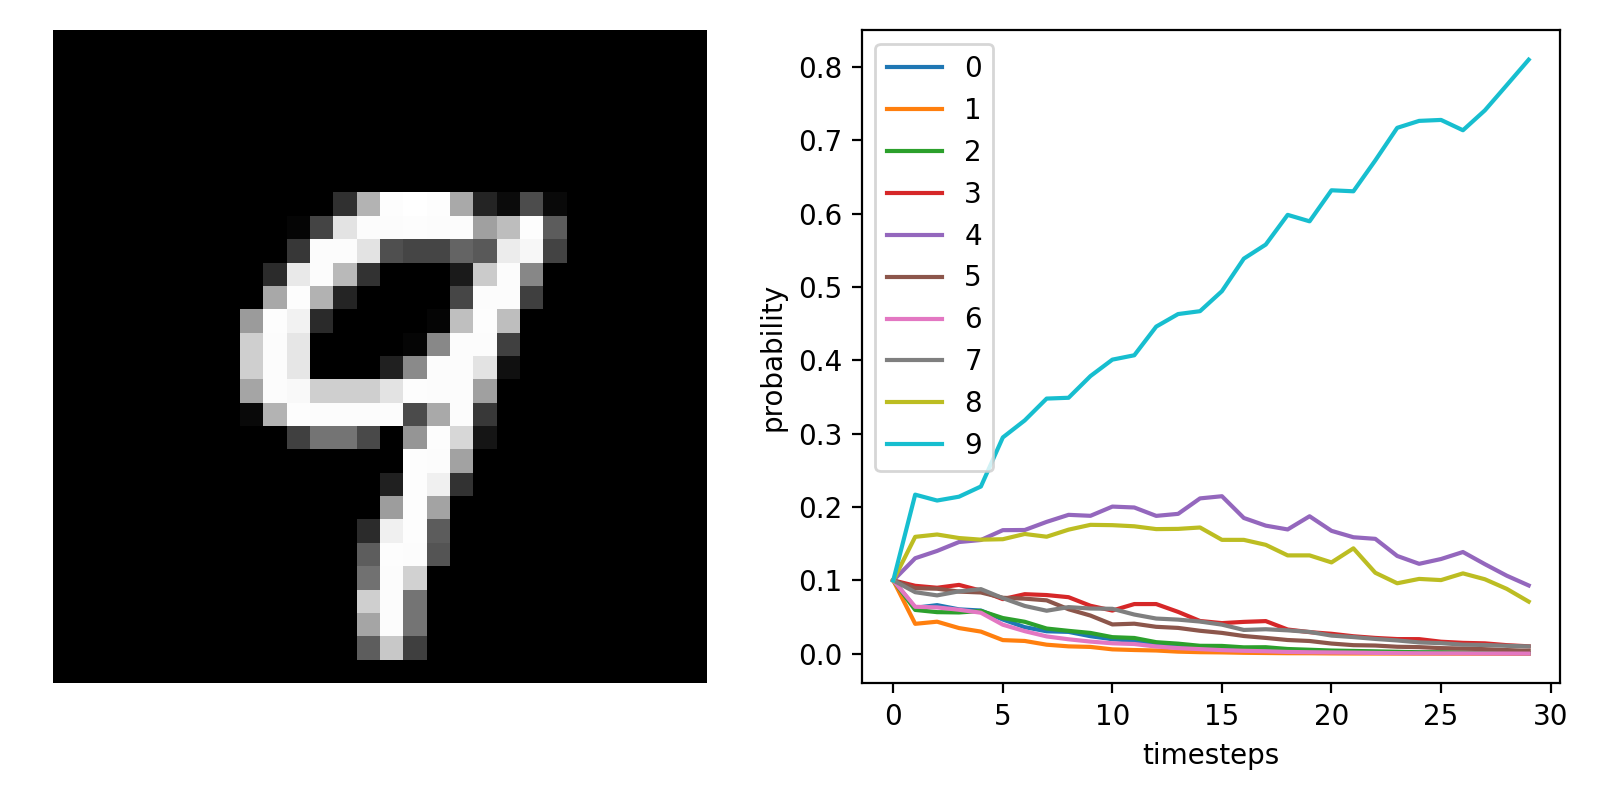
\includegraphics[width=\textwidth]{images/Figure_9.png}
\caption{Prediction of number 9} \label{fig4}
\end{figure}

The results show that Nengo has a great API and support for computations as it uses TensorFlow backed. One of the framework's cons is that It does not support other training approaches like spike timing-dependent plasticity (STDP).

\subsection{ Oscillator CPG model}
Reciprocal half-center oscillator "chess-clock" model implemented in MATLAB by Yakovenko\cite{ref27} chosen to be a baseline model. It consists of 4 artificial neurons(sell  Fig.~\ref{fig4}) interconnected with each other using a leaky integrator so that a spike of one neuron would limit activation of other neurons. This approach allows the model to produce cyclic pasterns of flexor and extensor. The model represented as a system of differential equestrians (1,2)

\begin{figure}
\centering
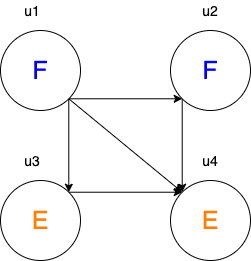
\includegraphics[scale=0.7]{images/model_diagram.png}
\caption{Model Diagram} \label{fig4}
\end{figure}

\begin{equation}
\dot{x}=x_{0}+G_{u} u+G_{x}^{\mathrm{UL}} x+\left.G_{x}^{\mathrm{BL}}(1-x)\right|_{x>0}
\end{equation}
\begin{equation}
G_{x}^{\mathrm{UL}}=I r_{\mathrm{leak}}
\end{equation}

where $G_u$ matrix represents gains of input signals
$u, G_x$ matrices represent the strength of unilateral
and bilateral connections between elements of the
pattern generator with the internal states x that
have the constant bias $x_{0}$. and where $I$ is the identity matrix, $r_{\mathrm{leak}}$ is the constant
that determines intrinsic state-dependent feedback

We want to find our model's parameters to closely correspond to the characteristics of the phase duration as was empirically obtained for a cat dataset. We compute the activation peaks of model spikes by mesuring the distance between the maximum excitement of neurons. The task is to optimize the root mean square value (RMS) distance between ground truth phase duration characteristic and received from the model using  the Nelder-Mead simplex (direct search) method. 

This model is simple but could accurately reproduce experimental results
($R_{swing}^2$ and $R_{stance}^2$  are 0.915 and 0.999, respectively). But even in this case simple method to approximate solutions of ordinary differential equations Runge–Kutta (fourth-order) could take up to several minutes to converge. 

\section{Summary and Future Work}
At the current stage, we mostly get familiar with Nengo framework, basic SNNs implementation, and setup baseline model in MATLAB. Furthermore, now ready to start experimenting with Nengo architecture to recreate the brain CPG system for one muscle flexor and extensor but using SNNs. The future step would be to compare results with the baseline model

%
% ---- Bibliography ----
%
% BibTeX users should specify bibliography style 'splncs04'.
% References will then be sorted and formatted in the correct style.
%
% \bibliographystyle{splncs04}
% \bibliography{mybibliography}
%
\begin{thebibliography}{99}

%%%%%%%%% Checked
\bibitem{ref1}
Ijspeert AJ. Central pattern generators for locomotion control in animals and robots: a review. Neural Netw. 2008 May;21(4):642-53. Epub 2008 May 14. PMID: 18555958.
\doi{10.1016/j.neunet.2008.03.014}

\bibitem{ref1_2}
Hodgkin AL, Huxley AF (August 1952). "A quantitative description of membrane current and its application to conduction and excitation in nerve". The Journal of Physiology. 117 (4): 500–44. PMC 1392413. PMID 12991237
\doi{10.1113/jphysiol.1952.sp004764}

\bibitem{ref2}
Hellgren, J., Grillner, S., Lansner, A. Computer simulation of the segmental neural network generating locomotion in lamprey by using populations of network interneurons. Biol. Cybern. 68, 1–13 (1992). 
\doi{10.1007/BF00203132}

\bibitem{ref3}
Yakovenko S, Sobinov A, Gritsenko V. 2018. Analytical CPG model driven by single-limb velocity input generates accurate temporal locomotor dynamics. PeerJ Preprints 6:e26734v2
\doi{10.7287/peerj.preprints.26734v2}

\bibitem{ref4}
Traven, H., Brodin, L., Lansner, A., Ekeberg, O., Wall ¨ en, ´
P.,  Grillner, S. (1993). Computer simulations
of nmda and non-nmda receptors mediated synaptic
drive: sensory and supraspinal modulation of neurons
and small networks. J. of Neurophysiology, 70(2),
695-709.

\bibitem{ref5}
Ijspeert, A.J.. (2001). A Connectionist Central Pattern Generator for the Aquatic and Terrestrial Gaits of a Simulated Salamander. Biological cybernetics. 84. 331-48. 
\doi{10.1007/s004220000211}

\bibitem{ref6}
Williams, T. L. (1992a). Phase coupling by synaptic spread
in chains of coupled neuronal oscillators. Science,
258, 662-665.

\bibitem{ref7}
Yu, Junzhi  Tan, M. Chen, Jian  Zhang, Jianwei. (2014). A Survey on CPG-Inspired Control Models and System Implementation. IEEE transactions on neural networks and learning systems. 25. 441-56.
\doi{10.1109/TNNLS.2013.2280596}

\bibitem{ref8}
Collins, J.J., Richmond, S.A. Hard-wired central pattern generators for quadrupedal locomotion. Biol. Cybern. 71, 375–385 (1994).
\doi{10.1007/BF00198915}

\bibitem{ref9}
Wang, W., Wu, Z., Shi, T. et al. Voltage-control oscillator based on Pt/C/NbOx/TiN device with highly improved threshold switching performances. Sci. China Phys. Mech. Astron. 62, 127821 (2019). 
\doi{10.1007/s11433-019-1463-y}

\bibitem{ref10}
Fukuoka, Yasuhiro \& Kimura, Hiroshi \&  Cohen, Avis. (2003). Adaptive Dynamic Walking of a Quadruped Robot on Irregular Terrain Based on Biological Concepts. I. J. Robotic Res.. 22. 187-202.
\doi{10.1177/0278364903022003004}

\bibitem{ref11}
Espinal A, Rostro-Gonzalez H, Carpio M, Guerra-Hernandez EI, Ornelas-Rodriguez M, Puga-Soberanes HJ, Sotelo-Figueroa MA, Melin P. Quadrupedal Robot Locomotion: A Biologically Inspired Approach and Its Hardware Implementation. Comput Intell Neurosci. 2016;2016:5615618. Epub 2016 Jun 29. PMID: 27436997; PMCID: PMC4942632.
\doi{10.1155/2016/5615618}

\bibitem{ref12}
Endo, G. \&  Morimoto, Jun \&  Matsubara, Takamitsu \&  Nakanishi, Jun \&  Cheng, Gordon. (2008). Learning CPG-based Biped Locomotion with a Policy Gradient Method: Application to a Humanoid Robot. I. J. Robotic Res.. 27. 213-228. 
\doi{10.1177/0278364907084980}

\bibitem{ref13}
Stone, James. (2018). Principles of Neural Information Theory: Computational Neuroscience and Metabolic Efficiency. 

\bibitem{ref14}
Rueckauer Bodo, Lungu Iulia-Alexandra, Hu Yuhuang, Pfeiffer Michael, Liu Shih-Chii(2017). Conversion of Continuous-Valued Deep Networks to Efficient Event-Driven Networks for Image Classification. Frontiers in Neuroscience, volume 11, pages 682.
\doi{10.3389/fnins.2017.00682}

\bibitem{ref15}
Pande, S., Morgan, F., Cawley, S. et al. Modular Neural Tile Architecture for Compact Embedded Hardware Spiking Neural Network. Neural Process Lett 38, 131–153 (2013). 
\doi{10.1007/s11063-012-9274-5}

\bibitem{ref16}
Hodgkin A., Huxley A. (1952). A quantitative description of membrane current and its application to conduction and excitation in nerve. J Physiol. 1952;117(4):500-544.
\doi{10.1113/jphysiol.1952.sp004764}

\bibitem{ref17}
Gerstner, Wulfram \& Wulfram, \& Kistler, \& M., Werner. (2002). Spiking Neuron Models: Single Neurons, Populations, Plasticity.
\doi{10.1017/CBO9780511815706}

\bibitem{ref18}
Moss, F. \& Gielen, Stan \& Gerstner, W.. (2001). A framework for spiking neuron models - the spike response model. 

\bibitem{ref19}
Izhikevich, E.M.. (2004). Which Model to Use for Cortical Spiking Neurons?. Neural Networks, IEEE Transactions on. 15. 1063 - 1070.
\doi{10.1109/TNN.2004.832719}

\bibitem{ref20}
Wu, Yujie \& Deng, Lei \& Li, Guoqi \& Zhu, Jun \& Shi, L.P.. (2018). Direct Training for Spiking Neural Networks: Faster, Larger, Better. 

\bibitem{ref21}
Rostro-Gonzalez, Horacio \& garcia, Pedro \& Trejo-Caballero, G. \& Garcia-Capulin, Carlos \& Ibarra-Manzano, Mario \& Avina-Cervantes, Juan \& Huitzil, Cesar. (2015). A CPG system based on spiking neurons for hexapod robot locomotion. Neurocomputing. 
\doi{10.1016/j.neucom.2015.03.090}

\bibitem{ref22}
Lele, Ashwin \& Fang, Yan \& Ting, Justin \& Raychowdhury, Arijit. (2020). Learning to Walk: Spike Based Reinforcement Learning for Hexapod Robot Central Pattern Generation. 

\bibitem{ref23}
Cuevas-Arteaga, Brayan \& Dominguez-Morales, Juan Pedro \& Rostro-Gonzalez, Horacio \& Espinal, Andres \& Jiménez-Fernandez, Angel \& Gómez-Rodríguez, Francisco \& Linares-Barranco, Alejandro. (2017). A SpiNNaker Application: Design, Implementation and Validation of SCPGs. Lecture Notes in Computer Science (including subseries Lecture Notes in Artificial Intelligence and Lecture Notes in Bioinformatics). 10305. 

\bibitem{ref24}
Gutierrez-Galan, Daniel \& Dominguez-Morales, Juan Pedro \& Perez-Peña, Fernando \& Jiménez-Fernandez, Angel \& s Linares-Barranco, Alejandro. (2019). NeuroPod: a real-time neuromorphic spiking CPG applied to robotics. Neurocomputing. 381. 
\doi{10.1016/j.neucom.2019.11.007}

\bibitem{ref24_1}
Frigon A, D'Angelo G, Thibaudier Y, Hurteau MF, Telonio A, Kuczynski V, Dambreville C. Speed-dependent modulation of phase variations on a step-by-step basis and its impact on the consistency of interlimb coordination during quadrupedal locomotion in intact adult cats. J Neurophysiol. 2014 May;111(9):1885-902. Epub 2014 Feb 12. PMID: 24523521; PMCID: PMC4044364.
\doi{10.1152/jn.00524.2013}

\bibitem{ref25}
Nengo example models
https://www.nengo.ai/examples/. 

\bibitem{ref26}
Hunsberger, Eric \& Eliasmith, Chris. (2016). Training Spiking Deep Networks for Neuromorphic Hardware. 
\doi{10.13140/RG.2.2.10967.06566}

\bibitem{ref27}
Yakovenko S. Chapter 10--a hierarchical perspective on rhythm generation for locomotor control. Prog Brain Res. 2011;188:151-66. PMID: 21333808.
\doi{10.1016/B978-0-444-53825-3.00015-2}

\end{thebibliography}
\end{document}

%\bibitem{ref_article1}
%Author, F.: Article title. Journal \textbf{2}(5), 99--110 (2016)

%\bibitem{ref_lncs1}
%Author, F., Author, S.: Title of a proceedings paper. In: Editor,
%F., Editor, S. (eds.) CONFERENCE 2016, LNCS, vol. 9999, pp. 1--13.
%Springer, Heidelberg (2016). \doi{10.10007/1234567890}

%\bibitem{ref_book1}
%Author, F., Author, S., Author, T.: Book title. 2nd edn. Publisher,
%Location (1999)

%\bibitem{ref_proc1}
%Author, A.-B.: Contribution title. In: 9th International Proceedings
%on Proceedings, pp. 1--2. Publisher, Location (2010)

%\bibitem{ref_url1}
%LNCS Homepage, \url{http://www.springer.com/lncs}. Last accessed 4
%Oct 2017

